\documentclass[tikz,border=0pt]{standalone}
\usepackage[T1]{fontenc}
\usepackage{lmodern}
\usepackage{microtype}
\usepackage{graphicx}
\graphicspath{{../template/}}
\usetikzlibrary{calc}
\definecolor{ink}{HTML}{1B1B1B}
\definecolor{muted}{HTML}{6E6A63}
\definecolor{paper}{HTML}{FAF8F3}
\definecolor{rule}{HTML}{D9D3C7}
\definecolor{card}{HTML}{FFFFFF}
%% Repository cover. Build:  pdflatex cover.tex  then rasterise cover.pdf
%% at 1280x640 (GitHub's social-preview size).
\begin{document}
\begin{tikzpicture}[x=1cm,y=1cm]
\clip (0,0) rectangle (16,8);
\fill[paper] (0,0) rectangle (16,8);

% ---- left block -------------------------------------------------------
\node[anchor=west, text=ink, inner sep=0pt]
  at (0.95,6.98) {\fontsize{7.4}{9}\selectfont\scshape University Physics Competition};
\node[anchor=west, text=muted, inner sep=0pt]
  at (0.95,6.62) {\fontsize{7.4}{9}\selectfont 48 hours \textperiodcentered\ two problems \textperiodcentered\ one paper};

\node[anchor=west, align=left, text=ink, inner sep=0pt]
  at (0.92,5.62) {\fontsize{26}{30}\selectfont\bfseries UPC Paper Toolkit};

\draw[rule, line width=0.5pt] (0.95,4.92) -- (7.10,4.92);

\node[anchor=north west, align=left, text=ink, inner sep=0pt, text width=6.15cm]
  at (0.95,4.70) {\fontsize{10}{14.6}\selectfont
  A \LaTeX{} project template that already compiles, and an agent skill
  distilled from the 74 gold-medal papers: the rules, the structure, and the
  judgement calls the judges reward.\par};

\draw[rule, line width=0.4pt] (0.95,1.52) -- (4.30,1.52);
\node[anchor=north west, text=muted, inner sep=0pt]
  at (0.95,1.40) {\fontsize{7.2}{10}\selectfont github.com/ziyepei06/uphysicsc-paper-toolkit};
\node[anchor=north west, text=muted, inner sep=0pt]
  at (0.95,1.08) {\fontsize{7.2}{10}\selectfont 2010--2025 \textperiodcentered\ MIT \textperiodcentered\ \LaTeX\, + Python};

% ---- single page, bleeding off the right edge -------------------------
\begin{scope}[rotate around={-3:(13.05,3.80)}]
  \fill[black, opacity=0.04] (10.62,0.46) rectangle ++(5.66,7.16);
  \fill[black, opacity=0.05] (10.57,0.52) rectangle ++(5.66,7.16);
  \fill[card] (10.52,0.58) rectangle ++(5.66,7.16);
  \begin{scope}
    \clip (10.52,0.58) rectangle ++(5.66,7.16);
    \node[anchor=north west, inner sep=0pt] at (10.73,7.52)
      {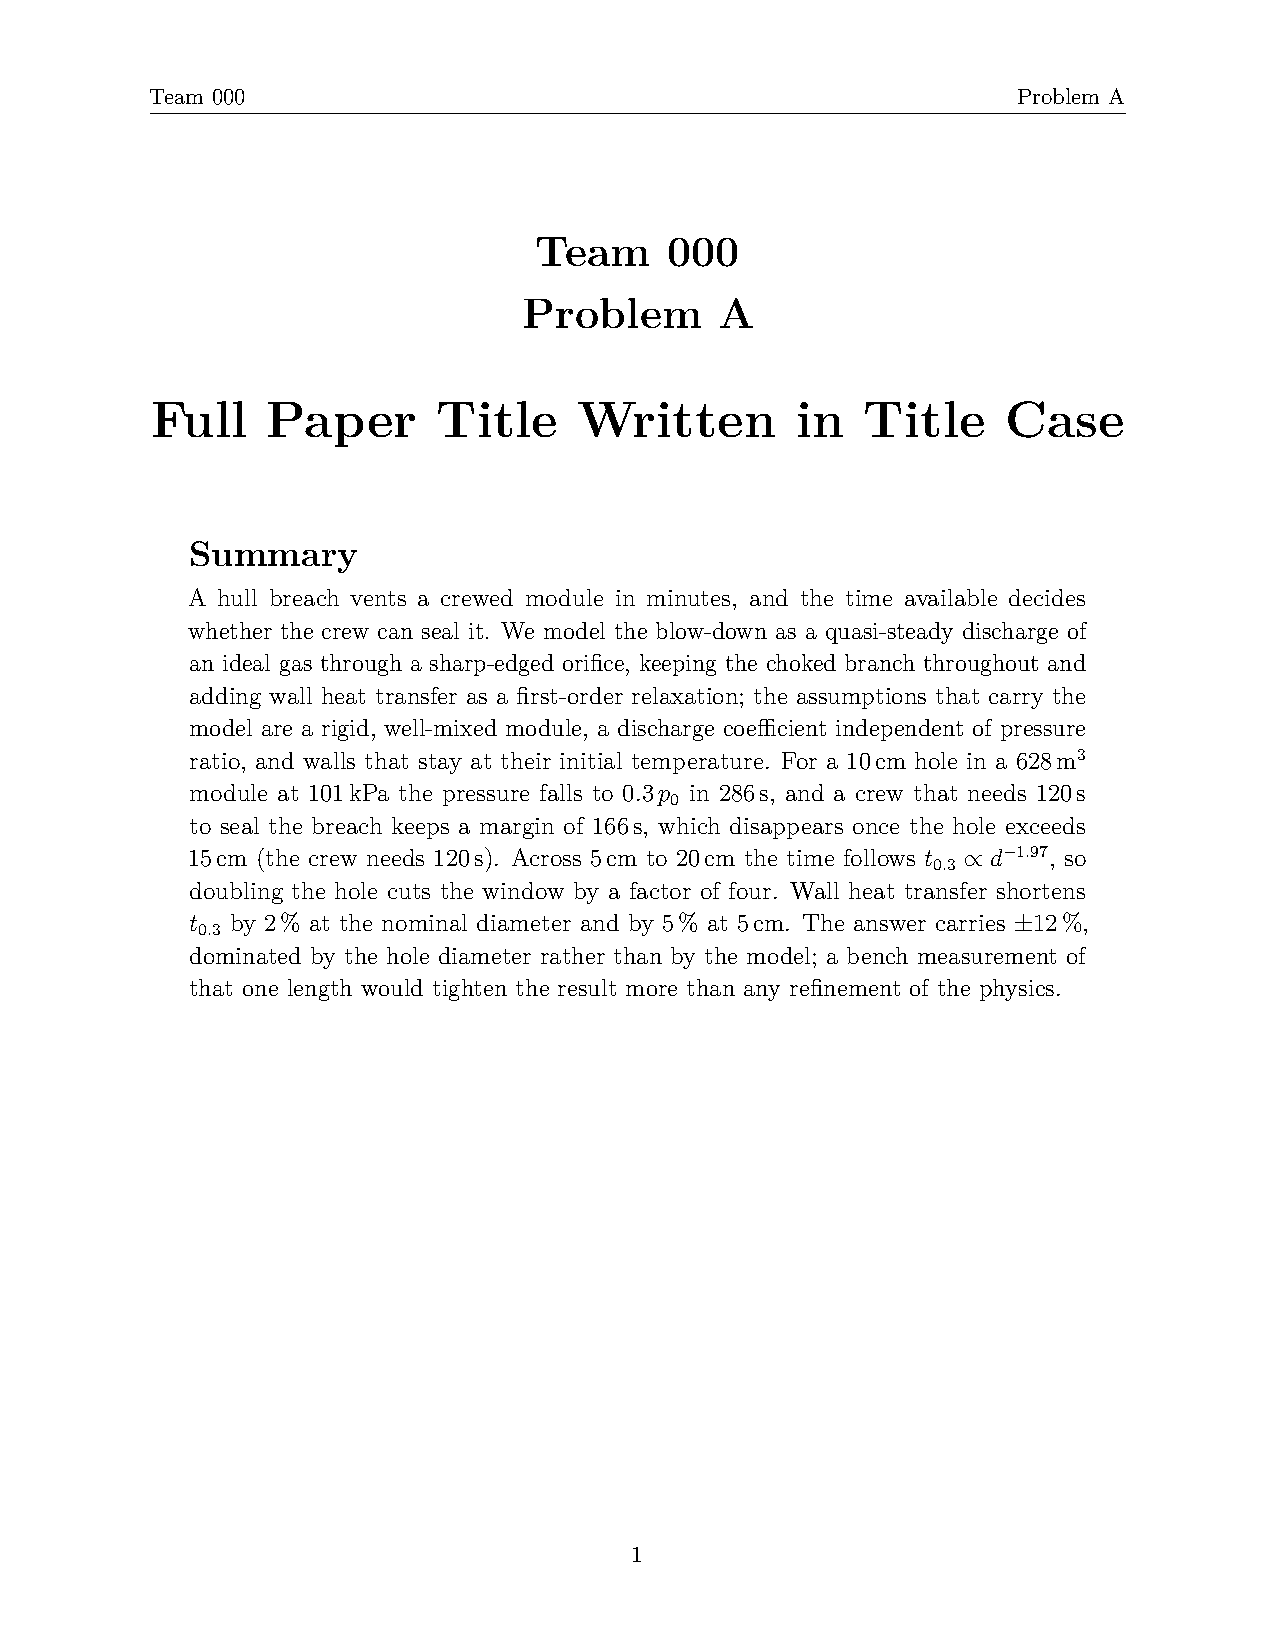
\includegraphics[page=1, width=5.24cm]{../template/000A.pdf}};
  \end{scope}
  \draw[rule, line width=0.4pt] (10.52,0.58) rectangle ++(5.66,7.16);
\end{scope}
\end{tikzpicture}
\end{document}
